\documentclass[a4paper]{article}
\usepackage[UTF8]{ctex}
\usepackage{amsmath,amsfonts,amssymb,amsthm}
\usepackage{graphicx}
\usepackage[left=10mm,right=10mm,top=10mm,bottom=10mm]{geometry}

%opening
\title{计算机科学中的数学基础--exercise2}
\author{陈昱衡 521021910939}
\date{\today}

\begin{document}

\maketitle


\section*{Warmup:Q6}
Some of the regions defined by n lines in the plane are infinite, while
others are bounded. What's the maximum possible number of bounded
regions?
\par 

\section*{Answer}
This question is a little different from the example from the textbook,but we can also try to solve the problem by visualizing the recurrent process. \par 
\begin{figure}[htb]
	\centering
	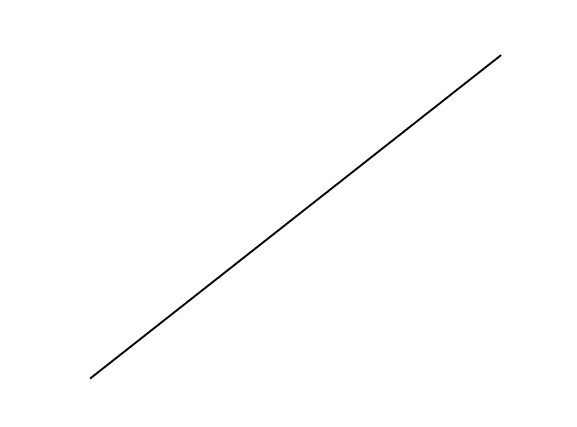
\includegraphics[scale=0.5]{Q61.png}
	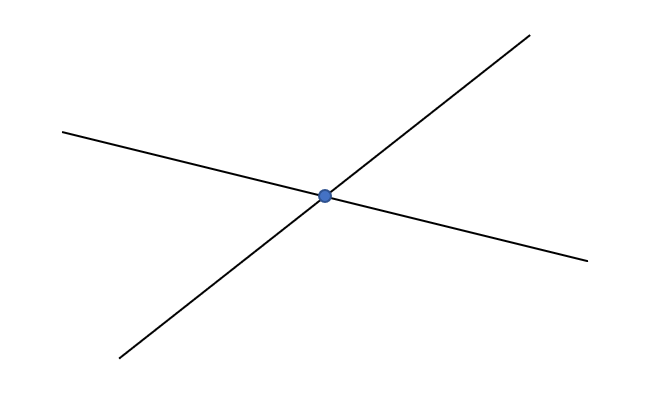
\includegraphics[scale=0.5]{Q62.png}
	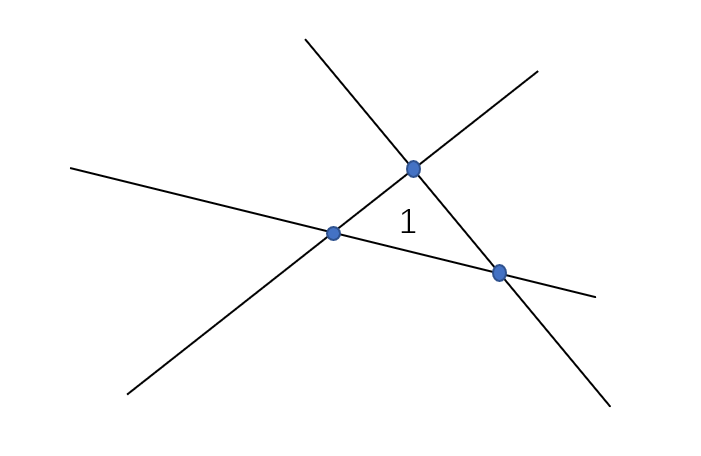
\includegraphics[scale=0.5]{Q63.png}
	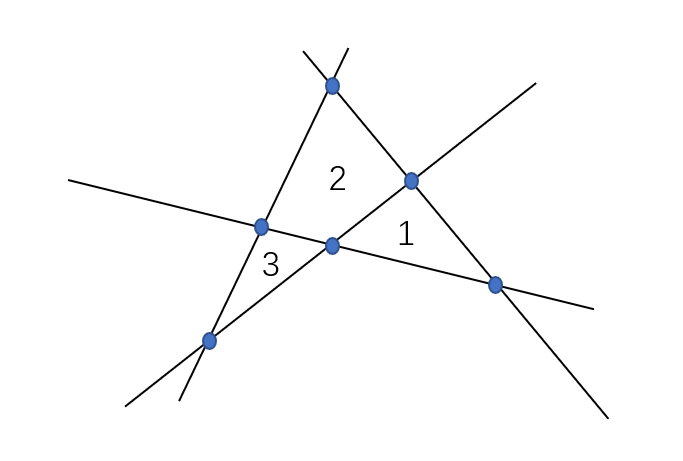
\includegraphics[scale=0.5]{Q64.png}
	\caption{Q6-demo}
\end{figure}
%\begin{figure}[htb]
%	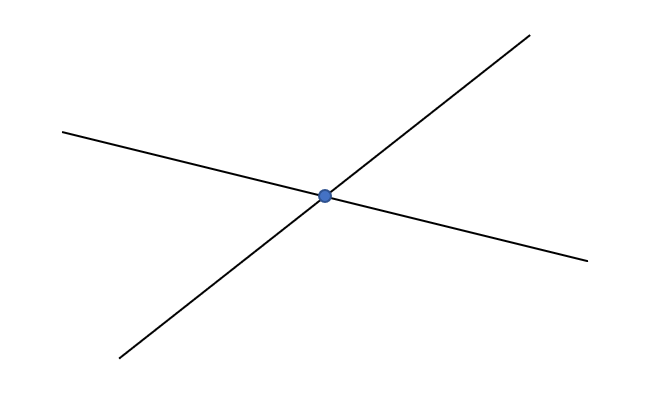
\includegraphics[scale=0.5]{Q62.png}
%	\caption{Q6-demo-2}
%\end{figure}\begin{figure}[htb]
%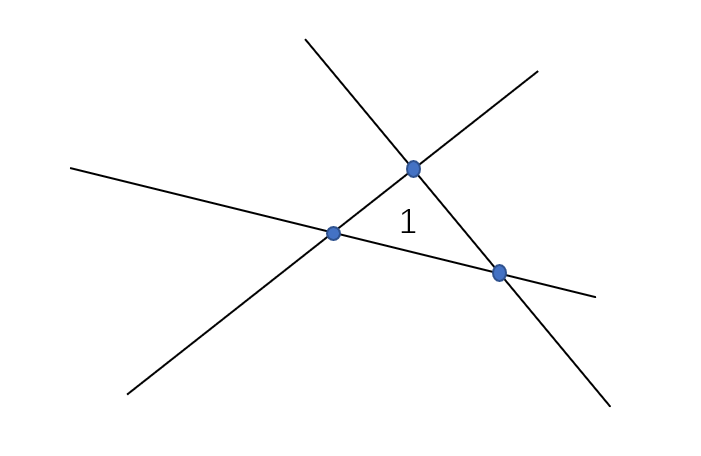
\includegraphics[scale=0.5]{Q63.png}
%\caption{Q6-demo-3}
%\end{figure}\begin{figure}[htb]
%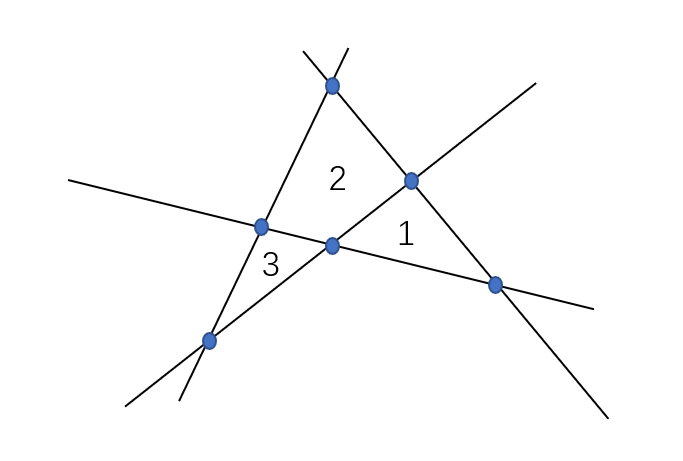
\includegraphics[scale=0.5]{Q64.png}
%\caption{Q6-demo-4}
%\end{figure}

So, we can kind of easily draw the conclusion that:the number of added bounded region equals the number of the lines which the new line intersect with minus one(in fact initially we can just ).So,we get the following recursive formula:


	\begin{align}
		&T_{n}=0 \quad (n=1) \\
		&T_{n}=T_{n-1}+n-2 \quad (n\ge2)
	\end{align}

We can get the answer by accumulating all the items together:
\begin{align}
&T_{n}=0 \quad (n=0) \\
&T_{n}=\frac{(n-1)(n-2)}{2} \quad (n\ge2)
\end{align}


\section*{Warmup:Q7}
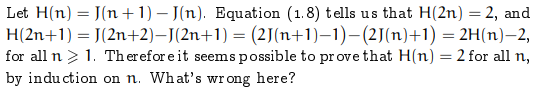
\includegraphics[scale=1.2]{Q7.png}
\section*{Answer}
We can easily notice that H(0)=1$\neq$2,so the foudation of the inductive method collapses.

\section*{Homework:Q8}
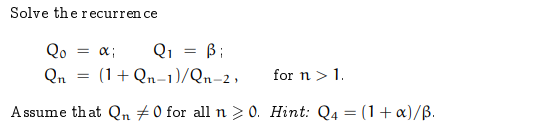
\includegraphics[scale=1.2]{Q8.png}
\section*{Answer}
Well,nothing had flashed across my mind when I was trying to solve the problem initially.What could I do was keeping calculating.Then,I got the answer.The series is periodic!\par 
\begin{align}
	&Q_{0}=\alpha \\
	&Q_{1}=\beta \\
	&Q_{2}=\frac{1+\beta}{\alpha} \\
	&Q_{3}=\frac{1+\alpha+\beta}{\alpha\beta} \\
	&Q_{4}=\frac{1+\alpha}{\beta} \\
	&Q_{5}=\alpha 
\end{align}


\section*{Homework:Q9}
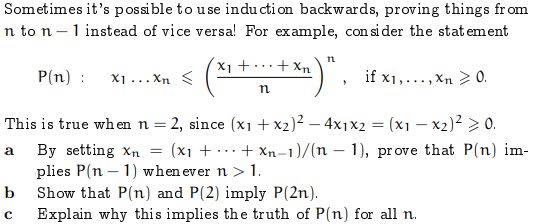
\includegraphics[scale=1.2]{Q9.png}
\section*{Answer}
\begin{enumerate}
	\item[(a)]
		If we want to prove P(n-1) using P(n),we can manage this by proving the following equation :\par 
		\begin{equation}
			x_{1}\cdots x_{n-1} (\frac{x_{1}+\cdots x_{n-1}}{n-1}) \le (\frac{x_{1}+\cdots x_{n-1}}{n-1})^{n}
		\end{equation}
	It's quite easy,as we can use the inequality:\par 
	\begin{equation}
		(\frac{x_{1}+\cdots x_{n-1}}{n-1})^{n-1} \ge (\frac{x_{1}+\cdots x_{n}}{n})^{n}
	\end{equation}
	\item[(b)]
	From P[n],we can get:\par
	\begin{equation}
		x_{1}\cdots x_{n}x_{n+1}\cdots x_{2n} \le ((\frac{x_{1}+\cdots+ x_{n}}{n})(\frac{x_{n+1}+\cdots+ x_{2n}}{n}))^{n}
	\end{equation}
then using P(2),we can further get :
	\begin{equation}
		((\frac{x_{1}+\cdots+ x_{n}}{n})(\frac{x_{n+1}+\cdots+ x_{2n}}{n}))^{n}
		\le
		(\frac{x_{1}+\cdots+ x_{2n}}{2n})^{2}
	\end{equation}
then the question got proved.\par 
	\item[(c)]
	Using the conclusion we got from (b),since we got P(2) now,then we can got P(4),using (a),we can get P(3).So,we can keep getting P($2^{k}$) using (b),and get P($2^{k-1}+1$) to P($2^{k}-1$).
\end{enumerate}

\section*{Homework:Q10}
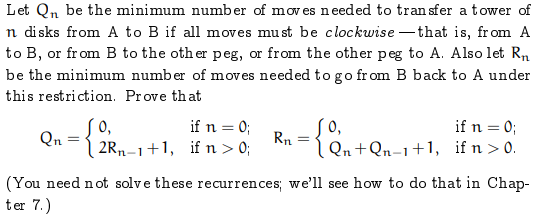
\includegraphics[scale=1.2]{Q10.png}
\section*{Answer}
To solve the problem,we are supposed to be aware that the process of moving the tower from A to B euqals to from B to C and C to A as well.Also,the process of moving the tower from A to C,from B to A,from C to B are the same,which is $R_{n}$ under the context.\par 
So,the first set of equations got proved,because we should move the upper n-1 plates from A to C which uses $R_{n}$,then move the biggest one from A to B which uses one step,finally move the n-  tower from C to B which is also at the cost of $R_{n}$.\par 
As to the second set of formula,we should move the upper n-1 plates from A to C,use $R_{n-1}$ steps,then the biggest one from A to B ,one step,then the n-1 tower from C to A,$Q_{n-1}$ steps,then move the biggest one to C,at last move the n-1 tower from A to C within $R_{n-1}$ steps.We got:
\begin{equation}
	R_{n}=R_{n-1}+1+Q_{n-1}+R_{n-1}+1
\end{equation}
With $Q_{n}=2R_{n-1}+1$ replacing $Q_{n}$,we got the right answer!.\par 

\end{document}
